% Downloaded MB
\begin{figure*}[t]
  \centering
  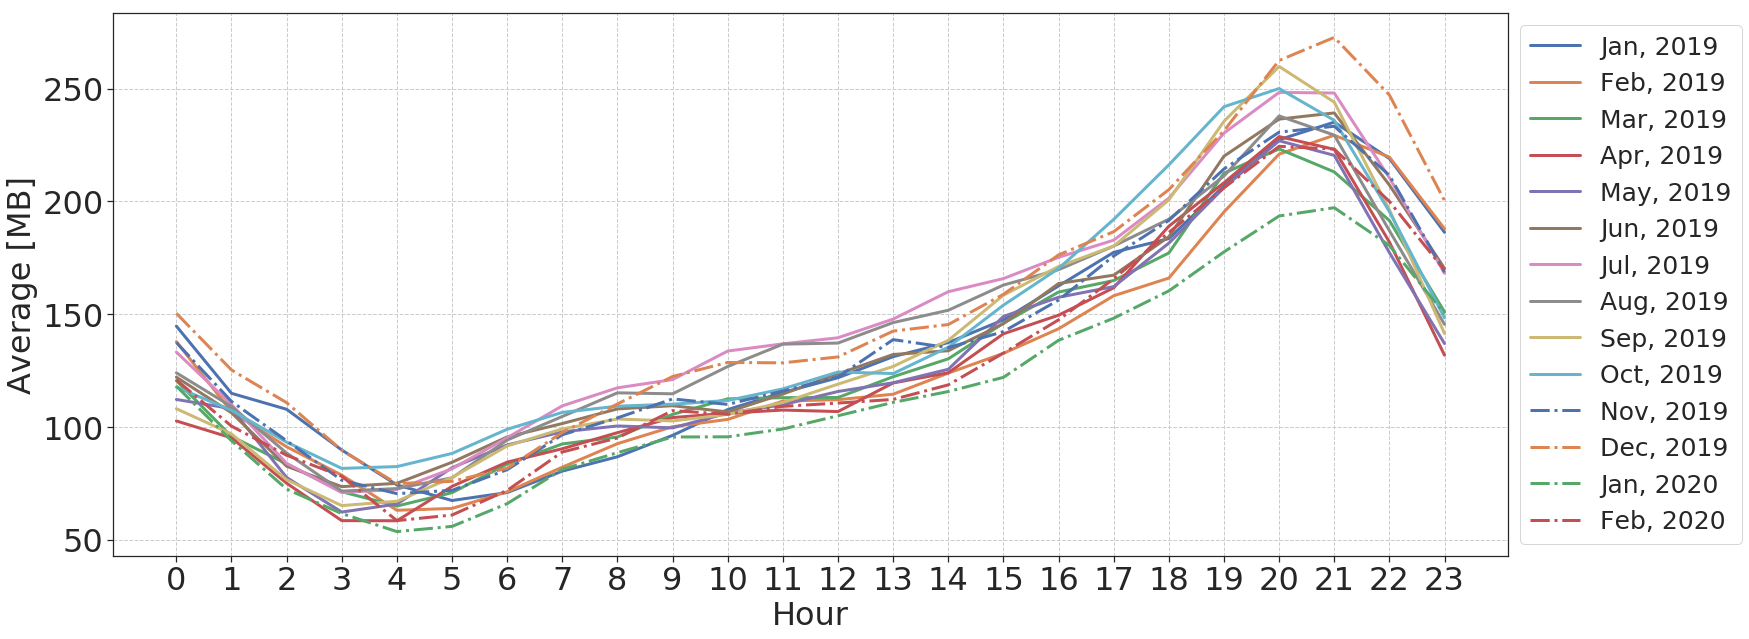
\includegraphics[width=.49\textwidth]{figs/wenjun/download_wdays_before.png}
  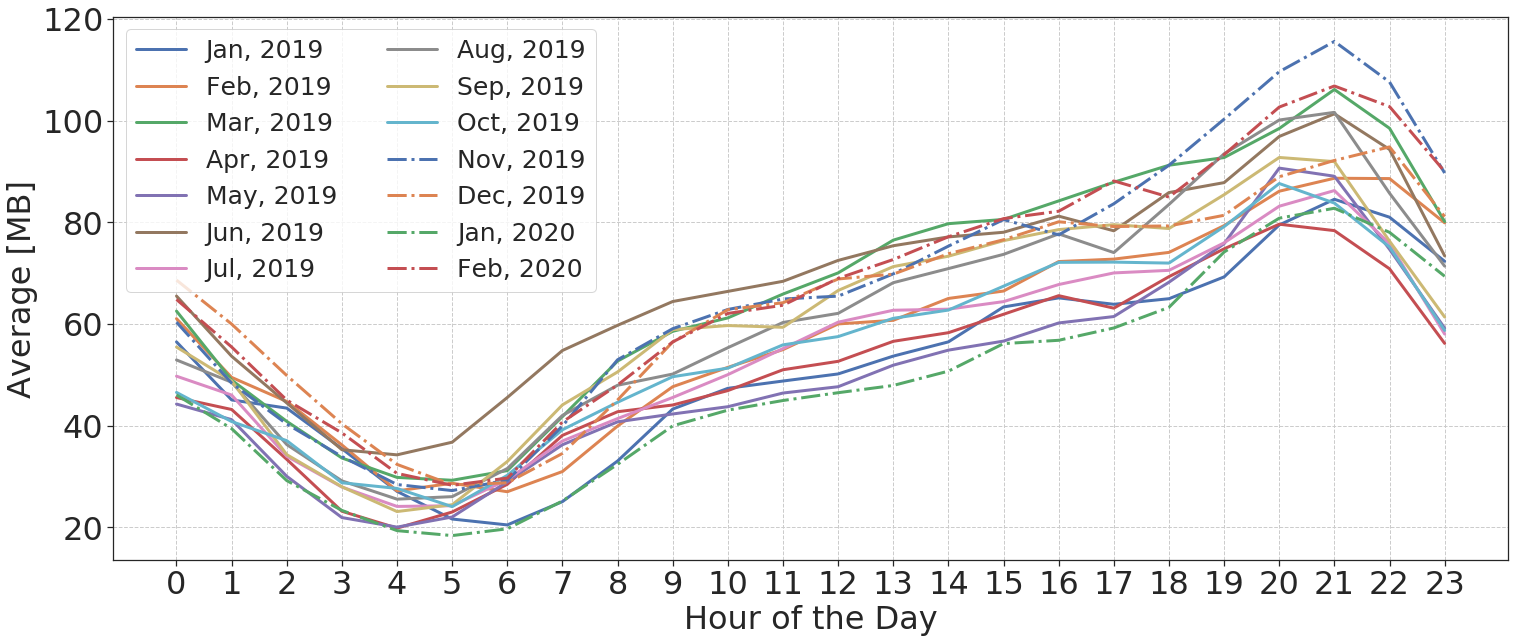
\includegraphics[width=.49\textwidth]{figs/wenjun/download_wends_before.png}
  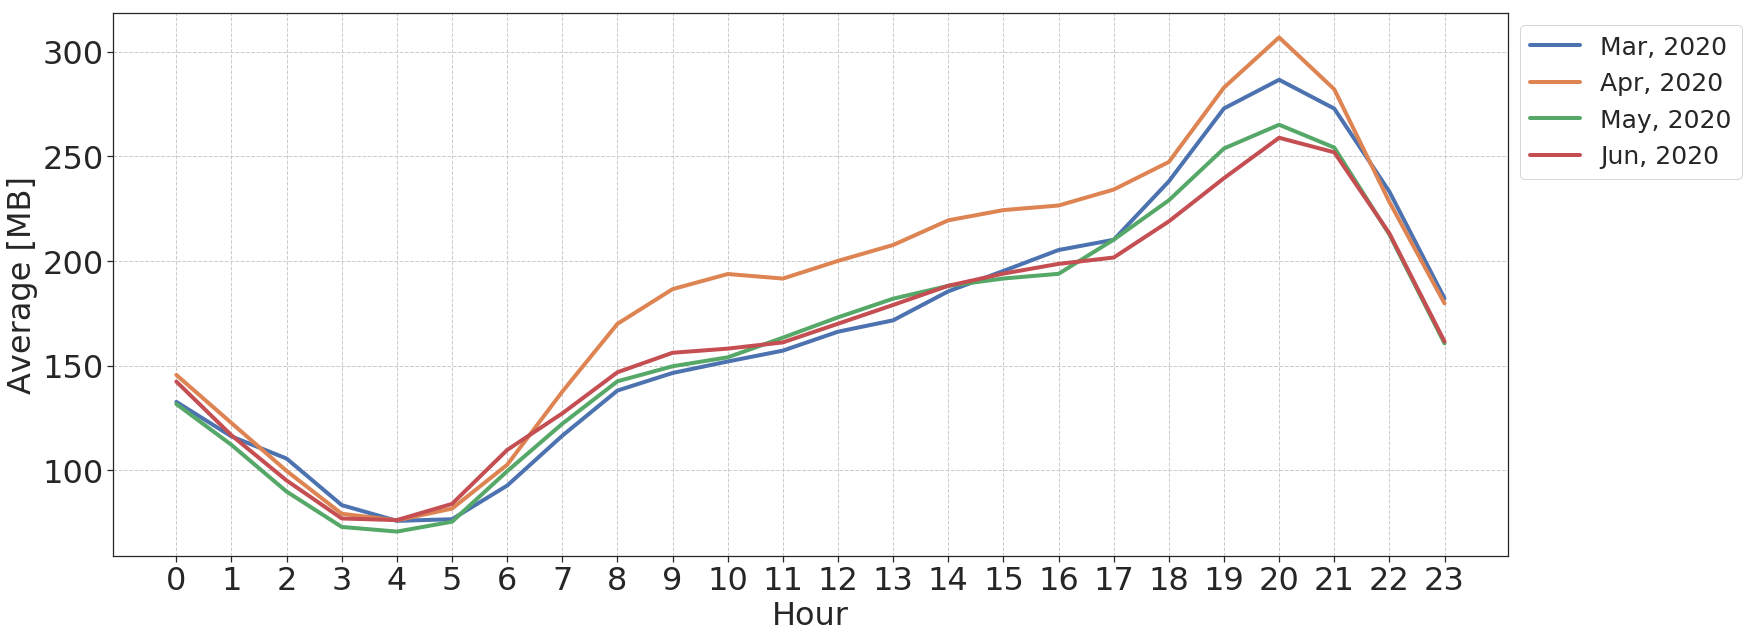
\includegraphics[width=.49\textwidth]{figs/wenjun/download_wdays_after.png}
  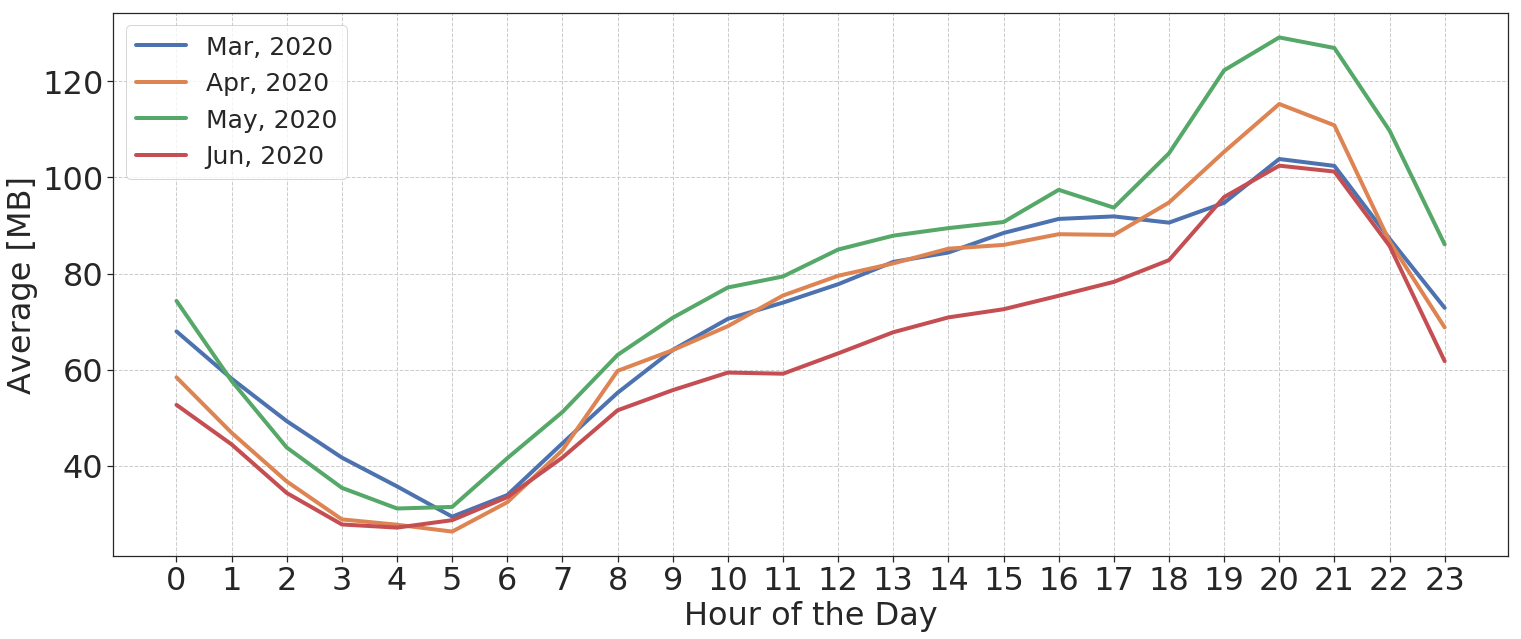
\includegraphics[width=0.49\textwidth]{figs/wenjun/download_wends_after.png}
  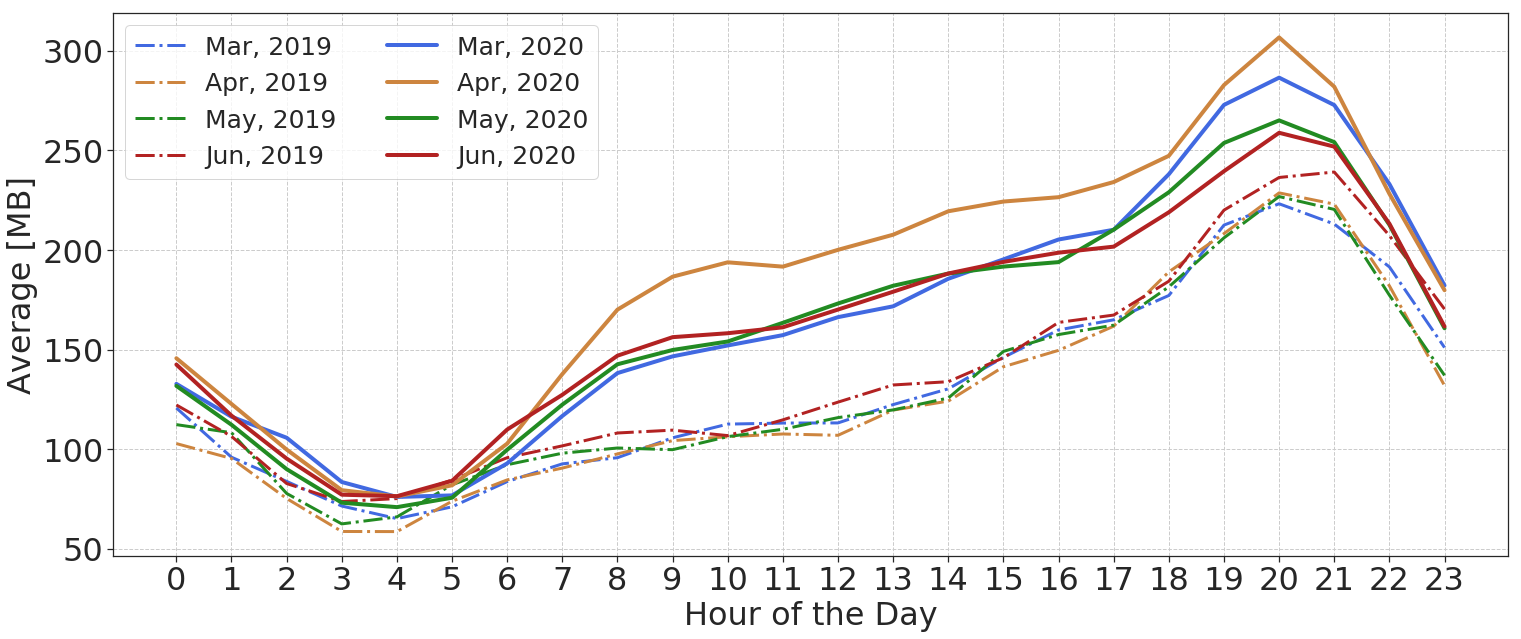
\includegraphics[width=.49\textwidth]{figs/wenjun/download_wdays_compare_36.png}
  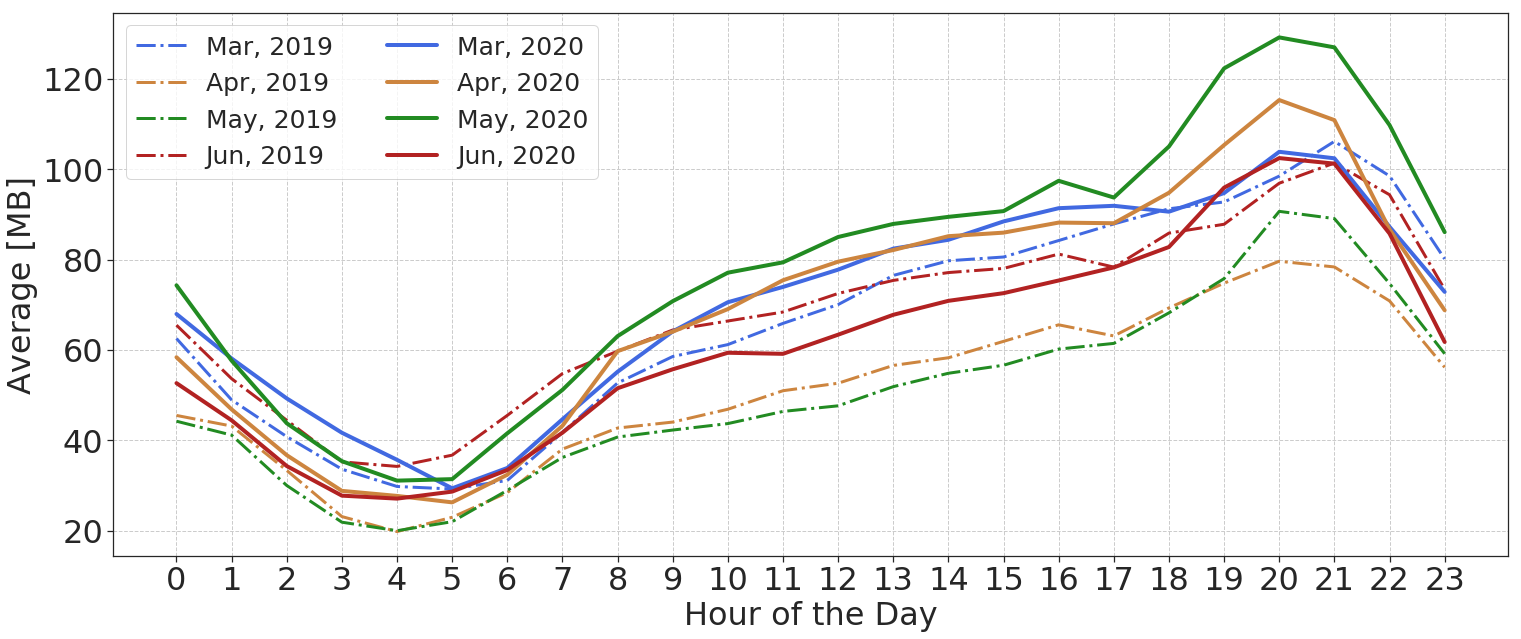
\includegraphics[width=0.49\textwidth]{figs/wenjun/download_wends_compare_36.png}

  \caption{Graphs related to Average Number of Download Data per Users over Hours on each Month. There is a peak between 18:00p.m. and 22:00p.m., which is the internet rush hour. The average download data per user over hour after COVID-19 is larger than that before COVID-19.}

  \label{fig:download-data-per-user-hours-fig}
\end{figure*}

% Uploaded MB
\begin{figure*}[t]
  \centering
  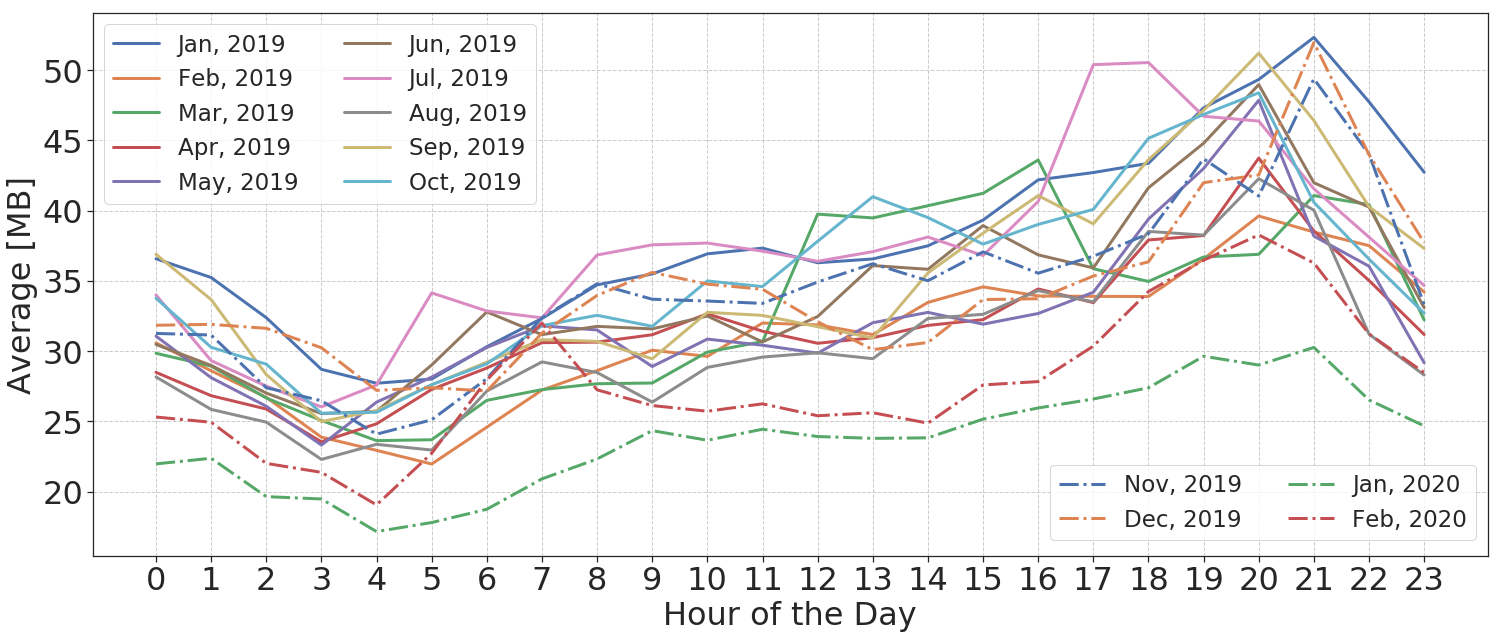
\includegraphics[width=.49\textwidth]{figs/wenjun/upload_wdays_before.png}
  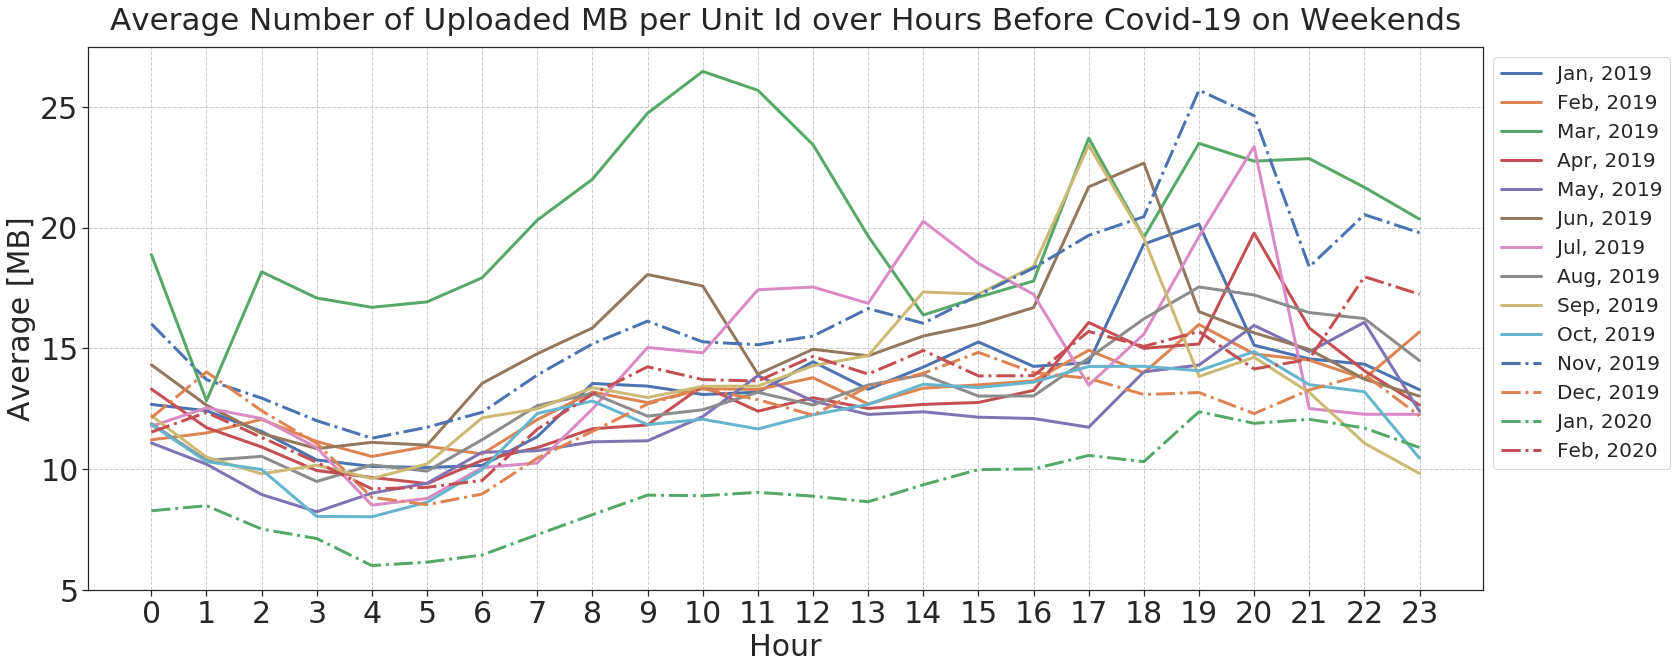
\includegraphics[width=.49\textwidth]{figs/wenjun/upload_wends_before.png}
  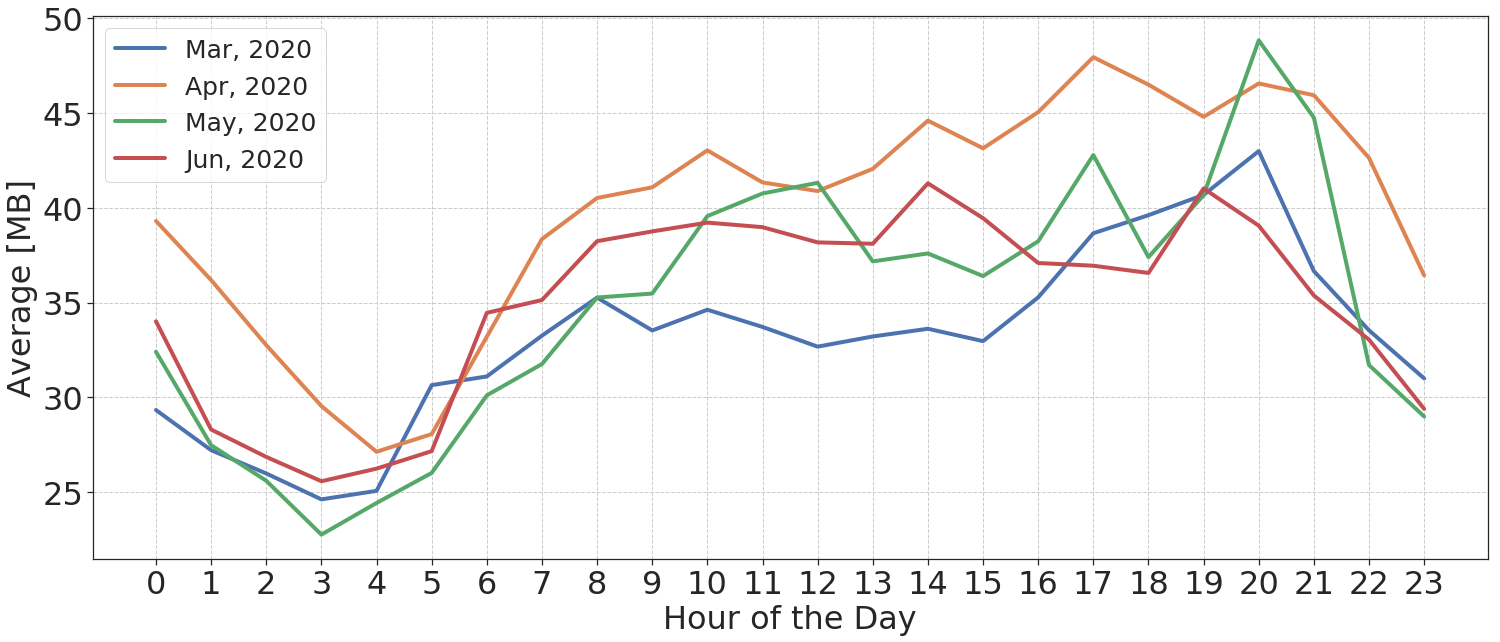
\includegraphics[width=.49\textwidth]{figs/wenjun/upload_wdays_after.png}
  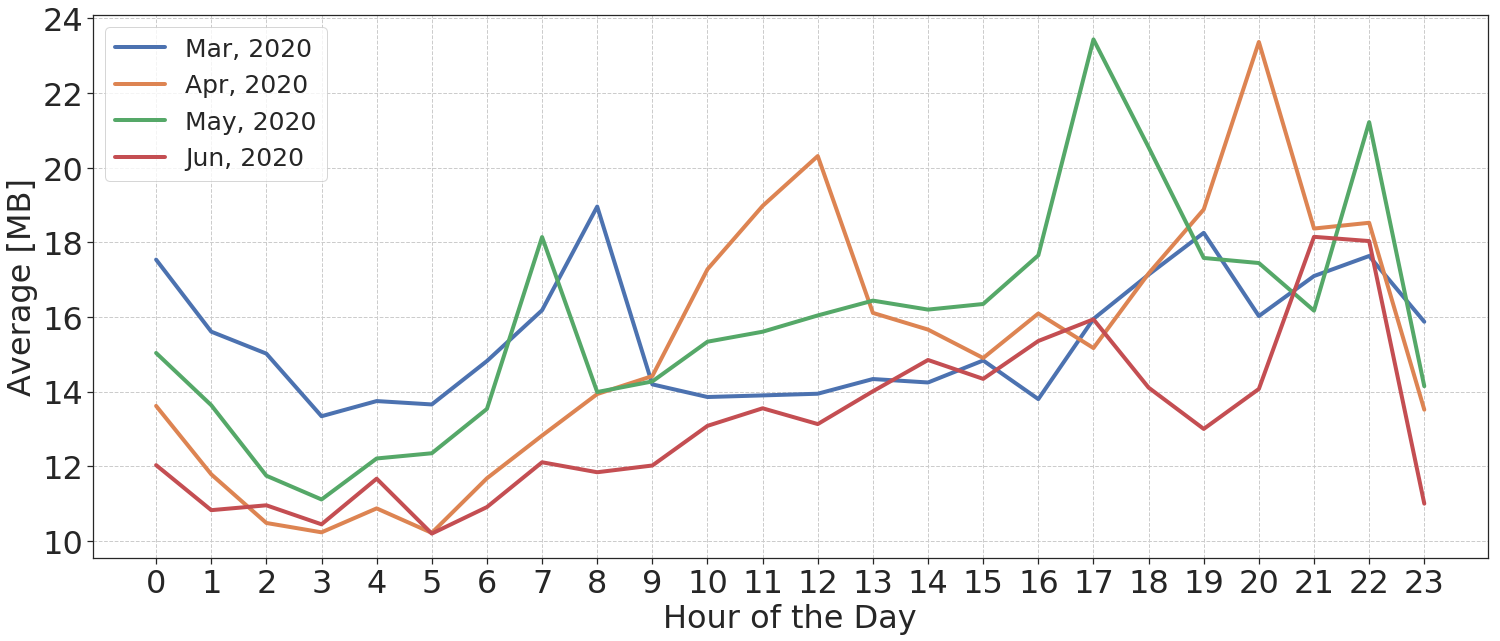
\includegraphics[width=0.49\textwidth]{figs/wenjun/upload_wends_after.png}
  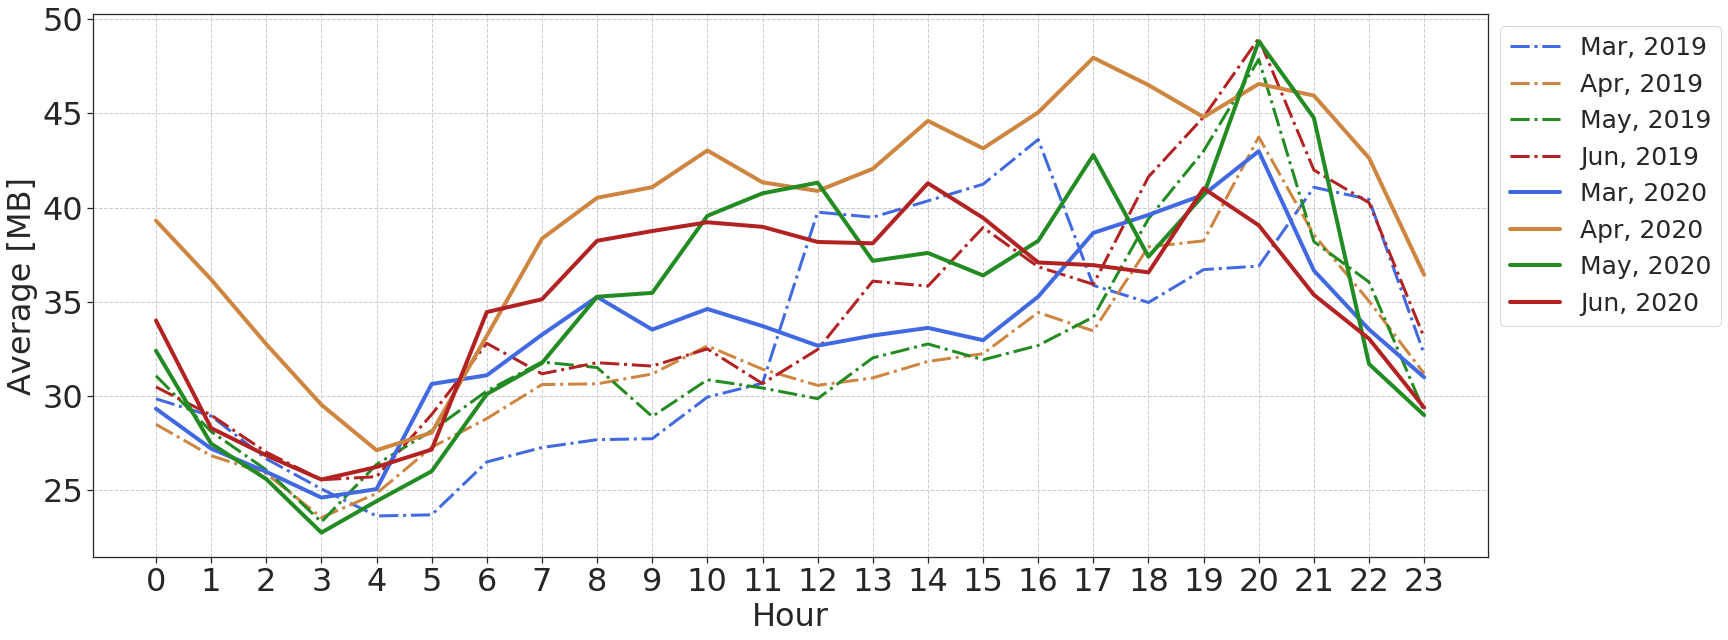
\includegraphics[width=.49\textwidth]{figs/wenjun/upload_wdays_compare_36.png}
  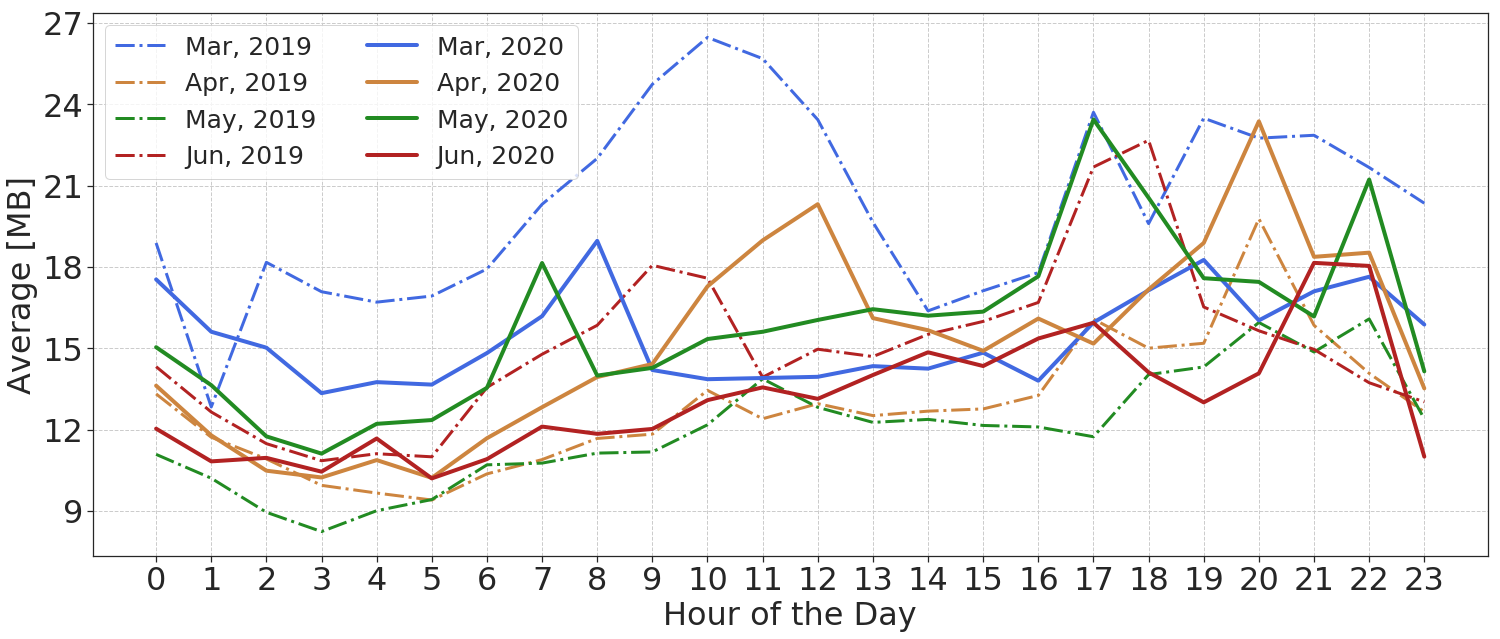
\includegraphics[width=0.49\textwidth]{figs/wenjun/upload_wends_compare_36.png}

  \caption{Graphs related to Average Number of Upload Data per Users over Hours on each Month. Compare with the pattern in average download data, the lines in the upload data graph are more fluctuating, especially the pattern for the upload data on weekends. In April and May, the average number of upload data per user over hour in 2020 is larger than that in 2019.}
  
  \label{fig:upload_data_per_user_hours_fig}
\end{figure*}

\subsection{Average Data Usage per Users over Hours on each Month}
We study the average data usage per users over hours on each month by comparing the average data usage on weekdays or weekends, and before COVID-19 or after COVID-19 based on both download data and upload data. 
% Since the recorded time in data set is finished in coordinated universal time, in order to get the time of download or upload event at local time, we add the time zone offset from the user profile to the recorded time.  We extract the year, month, and hour from the local time, and handle some special cases: (1) for hour, there is some location behind coordinated universal time and if the hour in local time is negative, add the value by 24. (2) For month, if the value of hour in local time is negative and the day is 1, we subtract the value of extracted month by 1 because it will be the last date of the previous month, and (3) for year, if the value of hour in local time is negative, the month is 1 and the day is 1, we subtract the value of extracted year by 1 since it will be the last date of the previous year. For the users, we focus on users who are present throughout the course of the study. We notice that the number of bytes that the customer transmitted from wired LAN devices to the internet for some users is the value of maximum integer. The possible reason is that the device measuring that value may be broken so we ignore all the users who have those values.


\subsubsection{Average Download Data per User}
\label{sec:download-data-per-user-over-hours}

% The download data is the number of bytes that the customer received from the internet to wired LAN devices and the Wi-Fi devices. 

As shown in the Figure \ref{fig:download-data-per-user-hours-fig}, we can find that the patterns of download data usage are the same on weekdays and weekends whether before COVID-19 or after COVID-19. There is a peak between 18:00p.m. and 22:00p.m., which is the internet rush hour \cite{internetrushhour}. People like to watch streaming video after work or dinner from YouTube, Netflix, and so on, and these streaming videos result in a huge amount of download data.

Moreover, according to the bottom figures in Figure \ref{fig:download-data-per-user-hours-fig}, the average download data per user over hour after COVID-19 is larger than that before COVID-19. 

On weekdays (the bottom left subfigure in Figure \ref{fig:download-data-per-user-hours-fig}), the gaps between average number of downloaded data per user from March to June in 2020 and those in 2019 from 7:00 a.m. to 22:00 p.m. are more obvious than those from 22:00 p.m. to 7:00 a.m. next day. The increase from 7:00 a.m. to 18:00 p.m. is because of work-from-home and online courses. Since the work-from-home mainly starts from April and May \cite{remotework}, the average number of downloaded data per user in April increases the most in 2020. The increase from 18:00 p.m. to 22:00 p.m. is due to gathering and social contact restriction, and then people are not allowed to hang out with friends and dine in at the restaurant after work \cite{lockdownsguide}. Instead, people need to stay at home. Watching streaming video or other recreational activities that require internet and cause a lot of downloaded data will be the first choice for most of the people. From 22:00 p.m. to 7:00 a.m. next day, it is time for sleep so the average number of download data per user after COVID-19 does not have too much difference with that before COVID-19. 

On weekends (the bottom right subfigure in Figure \ref{fig:download-data-per-user-hours-fig}), the increase of average downloaded data per user is a few in March, and there is a huge increase in April and May. In June, the average downloaded data per user in 2020 is not always larger than that in 2019. This pattern matches the policies related to COVID-19 in the United States: the height of restriction is at the end of March and the beginning of April, and some restrictions such as stay-at-home order is ended in the mid-late of May or in June at most of the states \cite{covid19restriction}. It means that in April and May, people need to stay at home and use internet the most. Since the restriction was started at the end of March, the average downloaded data per user was not affected too much, and in June, some of the restrictions end and people can restart the outdoor activities. Therefore, we can conclude that people use more internet and download more data because of COVID-19 and its related policies (e.g., lockdown, quarantine, work from home, etc.). 

\subsubsection{Average Upload Data per User}
\label{sec:upload-data-per-user-over-hours}

% The upload data is the number of bytes that the customer transmitted from wired LAN devices and Wi-Fi devices to the internet. 

As shown in the Figure \ref{fig:upload_data_per_user_hours_fig}, compare with the pattern in average download data, the lines in the upload data graph are more fluctuating, especially the pattern for the upload data on weekends. 

Similar to average download data per user, we compare the average number of upload data from March to June in 2020, which is the period after COVID-19, with that from March to June in 2019. According to the bottom figures in Figure \ref{fig:upload_data_per_user_hours_fig}, we can see that in April and May, the average number of upload data per user over hour in 2020 is larger than that in 2019 but in March and June, that is not the case. The reasons are the same as those for the average download data per user: the peak of shelter-in-place and stay-at-home are in the end of March and the beginning of April, and the restrictions are ended in the mid-late of May or in June at some states \cite{covid19restriction}. On weekdays, because of the policies such as work-from-home, the average upload data per user at daytime in April, May, and June 2020 are much larger than that in April, May, and June 2019. On weekends, the increase of average upload data per user is relatively smaller than that on weekdays. The possible reason is that weekend is a time to have a rest.  